\documentclass{article}
\usepackage{amssymb, amsmath}
\usepackage{graphicx}
\usepackage{epstopdf}
\usepackage[utf8]{inputenc}
\usepackage{mdwlist}
\usepackage[left=1cm, right=2cm, top=1.5cm, bottom=1.2cm]{geometry}
\epstopdfsetup{outdir=./}
\begin{document}

  \begin{enumerate*}
    \item []
    ID : 102062111, Name : Chih-Min Lin

    \item [1.]
    \begin{enumerate*}  
      \item [(a)] \text{}\\
      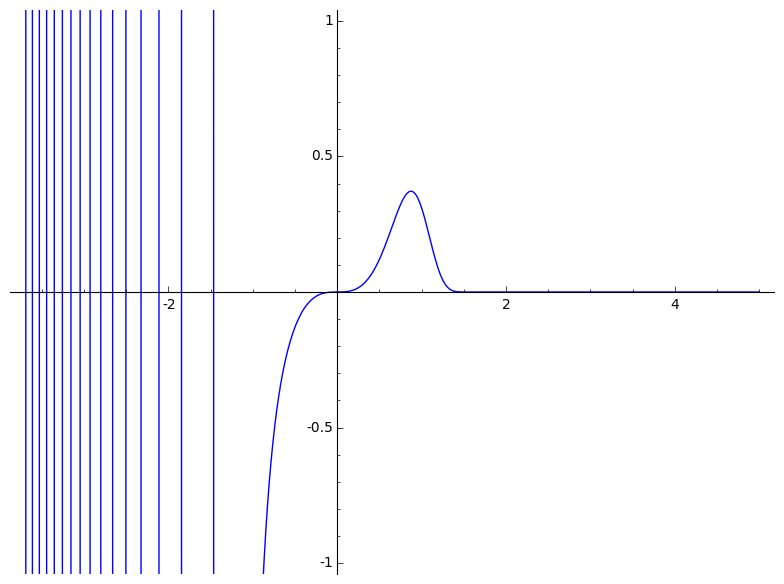
\includegraphics[width=0.7\textwidth]{/Users/chihmin/Desktop/science_computing/mid2_102062111/Q1_1.png}

	  \item [(b)] \text{}\\ 
      Because there are two functions, sin() and exp(), are too difficult to get the numerical result. If this equation has only 'exp()' or 'sin()', we could get the numerical result more easily.   
      
      \item [(c)] \text{}\\
      We can use 'numerical\_integral()' function to get approximated value of this integral. \\
      The result will return two values, left one is approximated value, and the other is an error estimate.

    \end{enumerate*}
    
    \item [2.]
    \begin{enumerate*}
      \item [(a)]
      $\because$ p is prime, and p is coprime between all integers from 1 to p except number p \\
      $\therefore \ phi(p)\ is\ p-1$ 
      
      \item [(b)]
      Obervation: \\
      $\phi(11) \times \phi(13) = \phi(11 \times 13)$ \\
      In my opinion, all distinct prime numbers p and q can be done by this observation, it looks really make sence. We should prove it in the next question.
      
      \item [(c)]
        \ 
        \begin{enumerate*}
          \item [(i)]
          Suppose we have distinct prime number p and q.
          \\

          \item [(ii)]
          $\because$ p is prime number, and q is also prime number \\
          $\therefore\ \phi(p) = p-1,\ \phi(q) = q-1,\ \phi(p)\phi(q)=(p-1)(q-1) = pq-p-q-1$
          \\

          \item [(iii)]
          $\because$ We observe "number set" coprime between $p \times q$ in range $[1,\ p\times q]$ : \\
          $\left\{ 1,\ 2,\ 3,\ ,\cdots\cdots,\ p \times q \right\}\ -$
          $\{p \times 1,\ p \times 2,\ \cdots\cdots p\times q \}\ -$
          $\{q \times 1,\ q \times 2,\ \cdots\cdots q\times p \}\ +$
          $\{p \times q\}$ \\ \\
          $\therefore$ The number of $PRIME\ SET\ =$ 
          $\phi(p \times q)=p \times q - p - q + 1$ 
          \\

          \item [(iv)]
          $\because(ii)\ is\ equal\ to\ (iii)$ \\
          $\therefore\ the\ equation\ holds.$
           
        \end{enumerate*}
         
      \end{enumerate*}

      \item [3.]
      \begin{enumerate*}
        \item [(a)]
        Use is\_prime() function to check whether a number is prime or not.\\
        Sample code : is\_prime(2**1279-1) \\
        Result : $2^{1279-1}$ is prime number
        
        \item[(b)]
        If values of a and p are really large, operations of calculating the result of $a^{p-1}\ \%\ p$ will cost a lot.

        \item[(c)] \
        \\
        Suppose we can find that $a^{n}\ mod\ p=1,\ n is positive integer$ \\
        If $a^{p-1}\ mod\ p=1$, then \\
        $a^{p-1}=a \times a \times a \times .... =a^n \times a^n \times .....$, $\frac{p-1}{n}$ will be positive integer

        Otherwise, the theory will not hold. \\
        Below is code implemented in SageMath environment : \\
        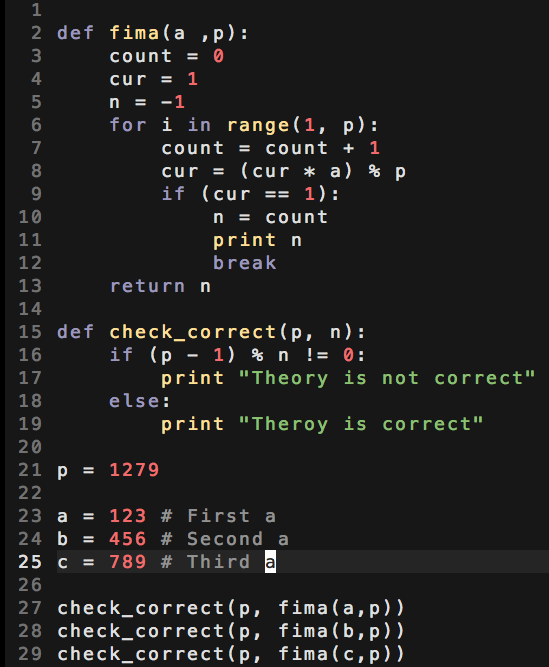
\includegraphics[width=0.5\textwidth]{/Users/chihmin/Desktop/science_computing/mid2_102062111/Q3_3.png} \\
        
        Below is the result of program running:\\
        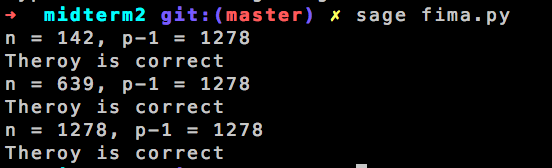
\includegraphics[width=0.5\textwidth]{/Users/chihmin/Desktop/science_computing/mid2_102062111/Q3_4.png}
         
    \end{enumerate*}
  \end{enumerate*}
\end{document}

